% Chapter 3
% add following line for typesetting from subfiles
% !TeX root = ../uet_thesis.tex
% !TeX root = ../uet_thesis.bbl
% !TeX root = ../references.bib
\chapter{Proposed Solution} % Write in your own chapter title
\label{Chapter3}
\lhead{Chapter 3. \emph{Proposed Solution}} % Write in your own chapter title to set the page header
%\section{Introduction}

%3)	Proposed Solution: Joint Brightness control and data transmission
%i)	PPM extension to multipulse block
%(a)	Combinatorial studies of MPPM
%ii)	MPPM for joint brightness control
%(a)	MPPM line codes for a simple case
%Algorithm for Implementation of MPPM code
%iii)	Decoder Algorithm
%(a)	Flow graph
%(b)	Matlab implementation
%(c)	Decoding example for case (5,2)
%iv)	Encoder Algorithm 
%(a)	Flow graph
%(b)	Matlab implementation

%(c)	Decoding example for case (5,2)

The requirement of joint brightness control and data transmission is met by proposing a novel line coding scheme. The proposed scheme does not require conventional dual modulation schemes based solution to meet the two objectives. The single modulation scheme pulse width modulates (PWM) the LED light source for brightness level and transmits data symbols at the same time with these PWM pulses. No additional analogue hardware is required. Simple iterative algorithms encodes and decodes the line coded symbols in linear time complexity. These algorithms are explained with examples. In following lines we start to solve the original problem from perspective of conventional line coding schemes, explaining the gradual development of proposed scheme.

\section{On-Off Keying In Visible Light Communication (VLC)}
%Before discussing the proposed scheme it would be useful to go through conventional line coding schemes in visible light communication scenario.
The simplest modulation technique for data transmission over optical networks is on-off-keying (OOK) that transmits data by turning the signal on for the signal bit \emph{one} and turning it off for signal bit \emph{zero}. This scheme can not be used to drive optical signal in visible light communication scenario because OOK does not possess a constant duty cycle (DC) or average value. Rather its DC average is a function of information bits statistics, how these are appearing in the signal. A light modulated with OOK will have flickering effect due to uneven distribution of ones and zeros. Besides that there is no way to control the brightness level. To understand this just imagine what happens when there is a long stream of ones, the light is illuminated to full brightness long as long as these ones keep on repeating. On the other hand when there is a long stream of zeros, light is essentially turned off. For any other random distribution of ones and zeros light intensity keeps on fluctuating in proportion to their presence in the data stream. Thus it is evident that OOK is not a proper solution to transmit data when illumination is the primary function of the light source.
%insert figure of an OOK driving signal here.

The light flickering problem can be cured by utilizing a constant average value line code such as  Manchester coding. In this case the light source intensity would remain constant for human eye perception, provided that the bit frequency is chosen high enough. To control the brightness level drive signal can be overridden by a DC offset signal. Though the brightness level can be set in this solution, however it is not a preferred scheme in 'all digital' system concept as it calls upon analogue hardware. It is also lesser power efficient and poses risk of LED chromatic shift \cite{dyble2005impact} \cite{levada2006high}. We are still seeking for a solution that has brightness control built in the encoding scheme itself.

\section{Pulse Position Modulation (PPM) \& VLC}
Another popular line coding technique for transmission over optical networks is pulse position modulation (PPM). It transmits data in the form of information blocks or frames. A PPM block consists of fixed number of time slots per frame, $n$, one of which contains a pulse and the rest remain at zero level. The position of the pulse within the frame determines the value of information to be transmitted. A 4-slot PPM frame can transmit a pulse in any one of the four possible slot positions. It provides four different combinations for a single 4-PPM frame. A combination denotes an information symbols. It means that the 4-PPM frame can transmit two information bits per frame. PPM is in fact a block coding scheme. A block code translate a group of input bits to a group of output bits. These two bit groups are called as information symbol $s_k$ and the encoded symbol $s_n$.
 %insert figure for PPM frame% 

\begin{figure}[t]
\centering
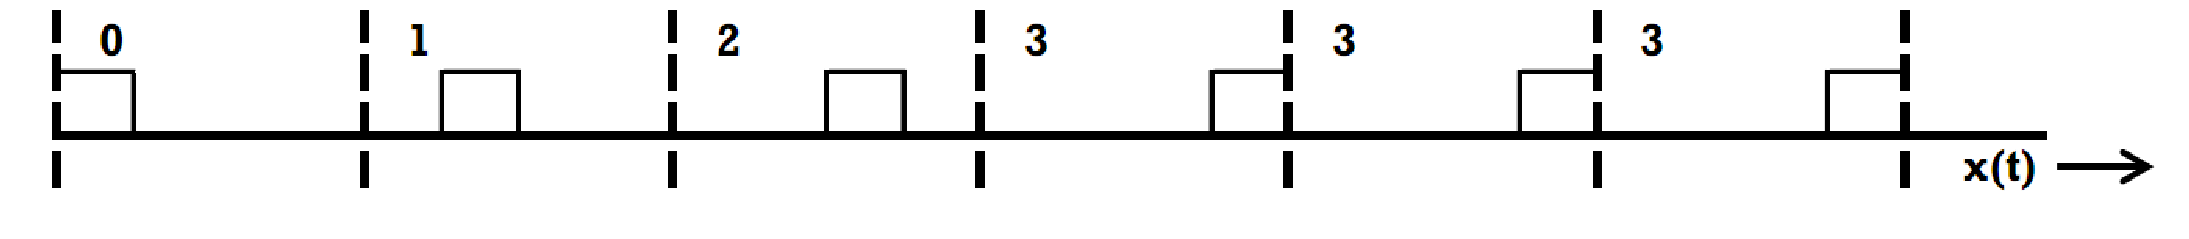
\includegraphics[width = \figwidth]{../Figures/PPM_frame}
\caption[PPM Signal]{A PPM signal transmits information symbols by position of the pulse in the frame. Digits 0,1,2 and 3 represent the information symbol being encoded.}
\label{fig:PPM_frame}
\end{figure}




A close inspection of PPM signal reveals that the average value of this signal remains fixed irrespective of the statistics of input bits. For a 4-PPM case, signal average value remains fixed at 25\% of the peak value at all times. To summarize above discussion, PPM is a constant average value or constant duty cycle (DC) technique that promises fixed illumination for the transmitting terminal light. In this way by employing PPM technique the flicker problem is solved. However the second problem of achieving control over brightness level remains unsolved. It is required that this DC average should be changeable without requiring external analogue hardware and without disturbing the data transmission.


%Heading PPM used for brightness control
%inser picture that shows PPM with 2,4 and 8 slot frames for brightness control
 This is an interesting question and to answer it we revisit the PPM encoding scheme. As noted above, average value of a PPM signal is $\frac{1}{frame~size}$. It shows the signal average value is inversely proportional to the frame size. That means the light source brightness can be changed by changing the frame size. For example if the 4-PPM is changed to 2-PPM, signal average value is doubled from quarter of the maximum voltage to the half of the maximum voltage level. Accordingly the information carrying capacity of a frame will be halved too, from 2-bits per frame to now only 1-bit per frame. Similarly by expanding the frame size from 4-PPM to 8-PPM, signal intensity would by halved from quarter of maximum to one eighth of the maximum drive voltage. The effect on information carrying capacity would be increase in bits per frame to 3-bits per frame. Though it is an effective technique that serves both the requirement of a modern LED based light source, that is the dimming control and the data transmission from a single line coding scheme. However even this scheme suffers from a few drawbacks. One, the frame size is not constant but is rather a function of brightness requirement of the light source. To decrease the brightness level, frame size must be increased and vice versa. It makes transmitter-receiver synchronization difficult once the brightness level is shifted to some other value. To comply with current industry standards the frame time should remain constant under all conditions. The second problem is that the coderate $\frac{1}{n}\lfloor \log_2(n) \rfloor$ drops with increase in frame size, $n$. Maximum code rate would be achieved for 2-PPM and then it is just half, i.e. one information bit transmitted for two bits of the line coded signal. For other brightness levels, frame size would have to be increased that will further deteriorate the coderate. Thirdly, brightness control is achieved in a non-linear fashion in steps of$\{\frac{1}{2}, \frac{1}{3}, \frac{1}{4}, \cdots \}$. Linear distribution of brightness levels would offer a better control. This discussion incites to search for a still better approach to the problem.

\section{Proposed Variable-Rate Pulse Position Modulation}
%Second thoughts to PPM
To look for a better encoding scheme we revisit the PPM and block codes. Consider all the $n^2$ codes that can be established by an n-bit block code. For didactic reason the example of $n=4$ is chosen. There are sixteen different possible four bit code words possible. These sixteen words can be grouped according to the number of \emph{ones} in a code word. In the described case of $n=4$ there can be total of five groups where each member of a certain group consists of either 0,1,2,3 or 4 ones. The codes in a group share a common property that the code duty cycle or average value is constant. It means if the light source is being modulated with one of the groups its light will remain fixed at one level associated with that group. By modulating with a different group of code words, brightness level can be shifted at the DC value of that very group. For the 4-bit code example, codes 0011 0110 1100 0101 1010 1001 are members of a group that all have 50\% duty cycle. If the group is changed to 0001, 0010, 01000, 1000 the brightness level will be 25\%.  Similarly by using other groups the brightness level can be set at at 0\%, 25\%, 50\%, 75\% or 100\%.  The code grouping according to the brightness levels is shown in table \ref{Ta:code_groupings}. The corresponding light source driving signal waveform is shown in figure \ref{Fig:line_codes}

\begin{table}
\begin{center}
\caption{4-Bit Codeword grouping according to brightness level.}
\begin{tabular}{|c|c|c|c|}
\hline\hline
Output Codeword&Input Symbol&Ones per Codeword& Brightness index\\
 &  $S_k$ & r &  $B_I$ \\
\hline\hline
0000 & 0 (00) & 0 & 0 \\ \hline
0001 & 0 (00) & 1 & 0.25 \\	
0010 & 1 (01) & 1 & 0.25 \\	
0100 & 2 (10) & 1 & 0.25 \\	
1000 & 3 (11) & 1 & 0.25 \\ \hline
0011 & 0 (00) & 2 & 0.5 \\	
0101 & 1 (01) & 2 & 0.5 \\	
0110 & 2 (10) & 2 & 0.5 \\	
1001 & 3 (11) & 2 & 0.5 \\	
1010 & 4 (100) & 2 & 0.5 \\	
1100 & 5 (101) & 2 & 0.5 \\ \hline
0111 & 0 (00) & 3 & 0.75 \\	
1011 & 1 (01) & 3 & 0.75 \\	
1101 & 2 (10) & 3 & 0.75 \\	
1110 & 3 (11) & 3 & 0.75 \\ \hline
1111 & 0 (00) & 4 & 1 \\ \hline
\hline
\end{tabular}
\label{Ta:code_groupings}
\end{center}
\end{table}


\begin{figure}[!htbp]
\centering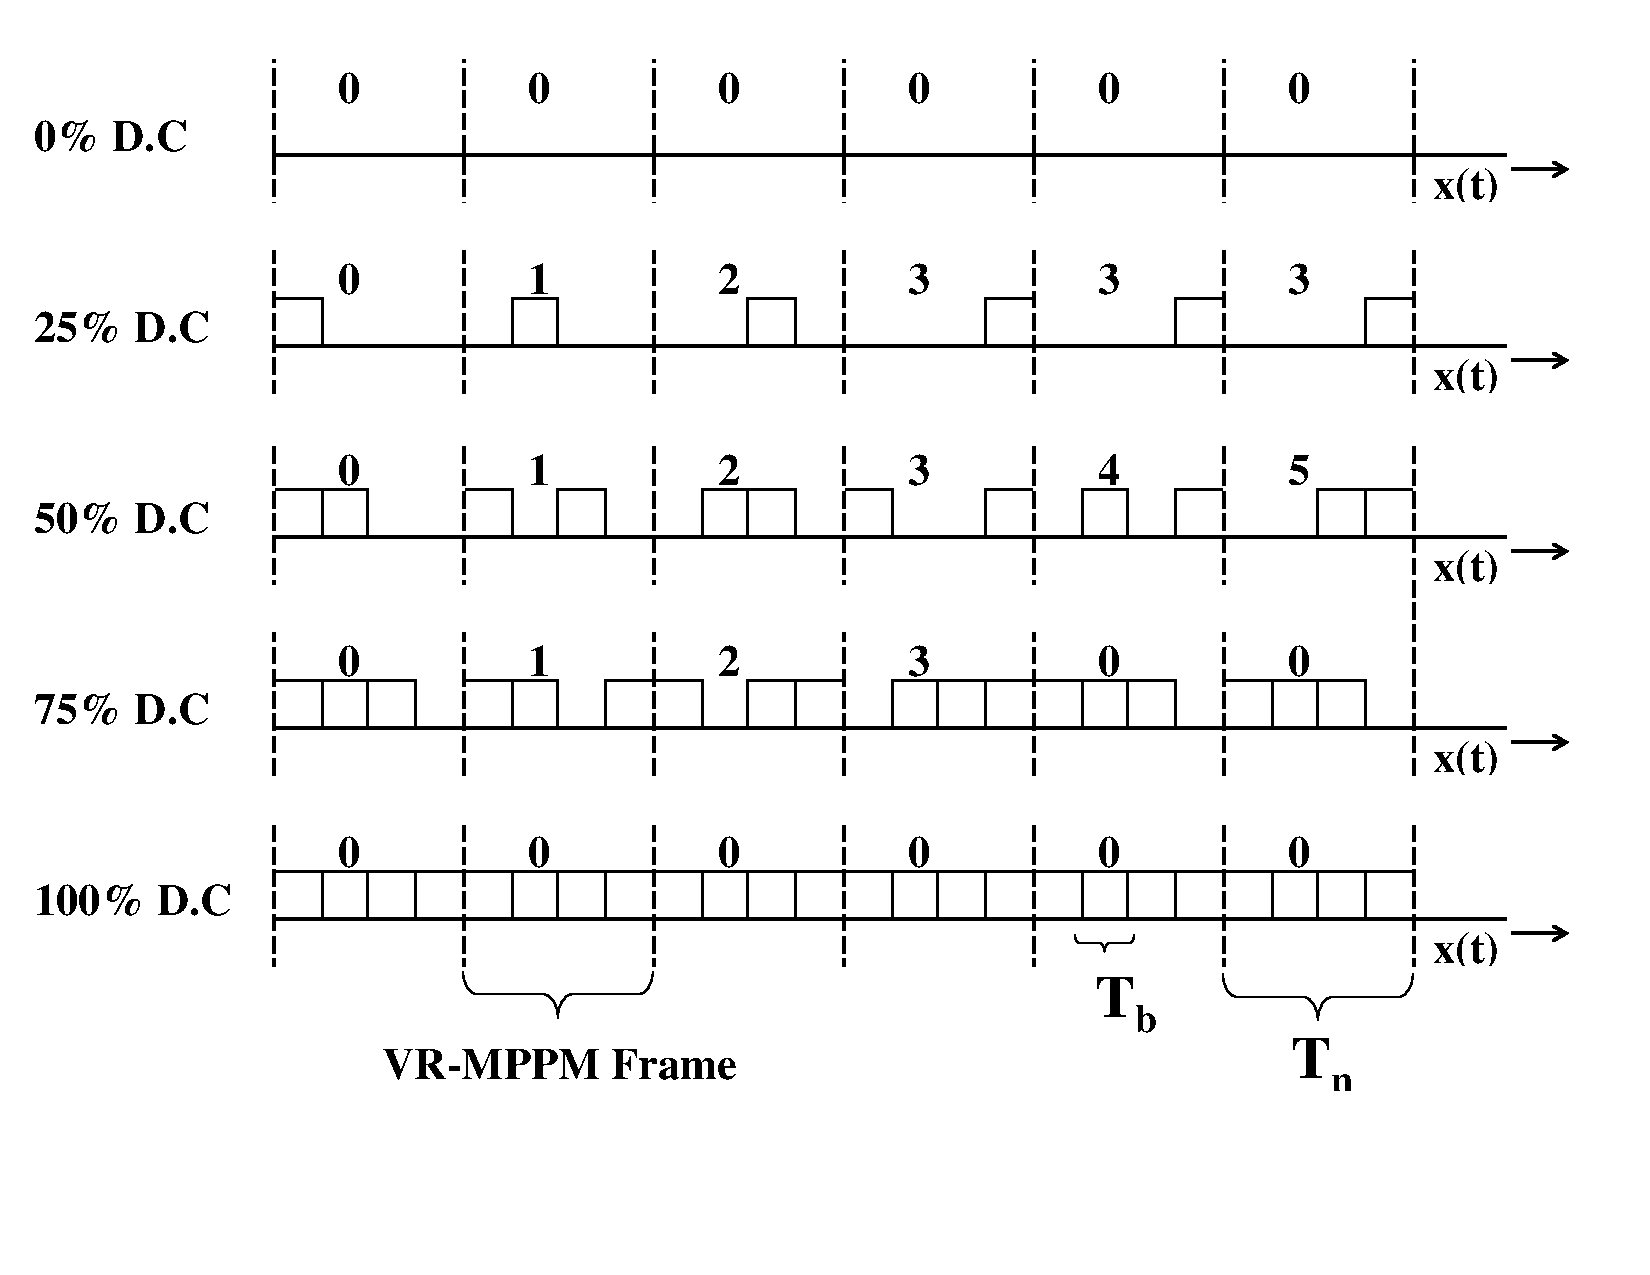
\includegraphics[width=\textwidth]{./Figures/line_code}
\caption{VR-MPPM encoded waveforms at different brightness indices }
\label{Fig:line_codes}
\end{figure}
%insert figure n=4 all possible codes 2^n 
%inser table (optional) with codes with number of ones and the brightness level
%insert waveform showing modulator output waveform

This is the solution presented in this thesis to achieve joint brightness control and data transmission of LED based light source. In above discussion, though the codes for 0\% and 100\% are valid as for as brightness control is concerned, however no information transmission is possible for these two cases. The former case (i.e. code 0000) applies to the situation when the light source is completely turned off and the later (code 1111) applies to the situation when light is fully turned on and there is no switching what so ever in the driving signal. From above discussion it can be inferred that the number of possible brightness levels with $n-bit$ codeword is $n+1$. The brightness level is identified by the number of 1's in a codeword that will now be represented by the variable $r$ such that $r \in \{0,1,2,\cdots,n-1,n\}$. An $n-bit$ long code word group with $r$ number of ones will be represented by symbol $(n,r)$. It represents that there are $r$ ones and $n-r$ zeros in the codeword. Here a new parameter \emph{Brightness Index} can be defined as:

\[\text{Brightness Index   } B_I = \frac{r}{n}\]
\begin{equation}
\begin{array}{cccl}

Where&&& \\
&r&=&\text{number of ones per codeword}\\
&n&=&\text{code word size}\\
	\end{array} 
\end{equation}

The value of brightness index takes values between zero and one with the two extremes being the case for light turned off and light turned on at full brightness when $r$ varied. By setting $n$ a fixed value as a system design parameter, a brightness control cum data transmission scheme evolves that has fixed frame size.


There is a relationship as how many different codewords are possible with a particular selection of $r$ at some fixed value of $n$. In fact this is similar to the classical problem of picking $r$ objects from $n$ total objects. The total number of combinations in this can be calculated by the combinational formula in equation \ref{eq:cominations}.

\begin{equation}
^nC_r = \frac{n!}{r! (n-r)!}
\label{eq:cominations}
\end{equation}•

The more combinations for a particular selection of $r$ the more number of information bits can be transmitted per frame size $n$. However the possible symbols from above formula do not necessarily form a fixed bit value. For instance the $n=4$ case discussed above does produce 4 different combinations for each value of $r=1$ and $r=3$. That can decode two information bits per symbol. However, for the case of $r=2$ there are six different possible symbols.  The effective bits that can be transmitted is still two. To transmitted three bits there must have been eight different symbols. Thus the effective number of transmitted bits per code word is calculated by equation \ref{eq:bits_per_codeword}:
\begin{equation}
Bits~per~codeword = \lfloor \log_2(^nC_r) \rfloor
\label{eq:bits_per_codeword}
\end{equation}•

Taking floor function means that some of the codewords need to be discarded. These extra codewords can be used for signalling information, such as receiver transmitter synchronization. 

Code rate for block codes is defined as the information bits transmitted per codeword bit. An $n$ bit long codeword with $r$ ones transmits at an effective code rate of $\frac{1}{n}\lfloor \log_2(^nC_r) \rfloor$. 

The proposed scheme can be thought as a variat of pulse position modulation that uses multiple pulses per frame instead of just one pulse. For this reason this coding scheme has been named as \emph{Variable Rate Multipulse Pulse Position Modulation (VR-MPPM)}. The acronym VR reminds that the code rate is not the constant but varies according to the selected brightness level.

The $2^n$ output symbols space is distributed among different brightness groups according to the following equation.
\[ 2^n=\binom{n}{0}+\binom{n}{1}+\underbrace{\cdots+ \binom{n}{r} +\cdots}_\text{r$\rightarrow$ 1's, (n-r)$\rightarrow$ 0's}+\binom{n}{n} \]

Though the assignment of input bit symbol to $2^n$ output codeword in table \ref{Ta:code_groupings} seems arbitrary at first glance, a novel algorithm has been designed in this thesis that performs this mapping in linear time complexity. This algorithm is explained in following passages.

\section{Algorithm}
The format of encoded word is similar in principle to the digit place value weightage function used in decimal and binary systems. Binary system assign place value to digits as $1,2,4,8,\cdots,so~on$ starting with least significant digit value equal to one. Similarly the decimal system assigns $1,10,100,1000,\cdot,~so~on$ as digit place values. However the proposed scheme has a small difference from these systems in that the place value for a digit is not fixed. Like binary system the digits used are 0's and 1's only. 

The place value system for a codeword of size $n$ with $r$ ones is discussed here. The weightage function is assigned to a \emph{digit} in the codeword as $\binom{i}{\rho}$, where $i$ and $\rho$ are two variables that index the digit in the code-word. The variable $i \in \{ 0,1,2,\cdots,n-1\}$ indexes the absolute  position of the digit in the codeword, zero being the index number for least significant digit. The variable $\rho \in \{1,2,\cdots,r\}$ indexes only the 1's in the codeword. The two possible values of $r = 0$ and $r = n$, though form valid codewords, are not considered here as these correspond to the two extreme conditions of light fully turned off or fully turned on and the communication is not possible in these cases. Thus for algorithm's purpose the values of $r$ is restricted to $r \in \{1,2,3,\cdots,n-1 \}$

%starting at 3:37 19-oct-2011
An information symbol $s_k \in \{0,1,2,\cdots,\lfloor \log_2(^nC_r) \rfloor \}$ encoded with n-bit long word with r-ones is represented by the trio $(n,r,s_k)$. As the code will be used to drive a line signal, the resulting wave form will have $r$ pulsed slots and $n-r$ non pulsed slots in a VR-MPPM frame. To encode the symbol $(n,r,s_k)$ the table \ref{tab:encode-decode} needs to be constructed. This table will be used to lookup the place value of the codeword digits. Each column represents the place value of a digit at index $i$. Each row modifies this place value depending upon the number of pulsed slots in the codeword. An entry $(i,r)$ in the table is constructed according to the relation:
\begin{equation}
\label{eq:placeValue}
    (i,\rho) = \left\{\begin{array}{cc}
    ^{i}C_\rho & i \geq \rho \\
	0 & i < \rho
\end{array}   \right.
\end{equation}

\begin{table*}[t]
\centering \caption{Symbol encoding and decoding matrix}
\begin{tabular}{c|c c c c c c c c} \hline \hline
$\rho \diagdown i$ & ${n-1}$ & ${n-2}$ & $\cdots$ & ${i}$& $\cdots$ & ${2}$ & ${1}$ & ${0}$ \\ \hline \hline
$n-1$ & $^{n-1}C_{n-1}$ & 0 & $\cdots$ & 0 & $\cdots$ & 0 & 0 & 0 \\ 
$n-2$ & $^{n-1}C_{n-2}$ & $^{n-2}C_{n-2}$ & $\cdots$ & 0 & $\cdots$ & 0 & 0 & 0 \\ 
\vspace{-6pt} \\
$\vdots$ & $\vdots$ & $\vdots$ & $\cdots$ & $\vdots$ & $\cdots$ & $\vdots$ & $\vdots$ & $\vdots$ \\ 
\vspace{-6pt} \\
$\rho$ & $^{n-1}C_{\rho}$ & $^{n-2}C_{\rho}$ & $\cdots$ & $^{i}C_{\rho}$ & $\cdots$ & 0 & 0 & 0 \\ 
$\vdots$ & $\vdots$ & $\vdots$ & $\cdots$ & $\vdots$ & $\cdots$ & $\vdots$ & $\vdots$ & $\vdots$ \\ 
\vspace{-6pt} \\
$2$ & $^{n-1}C_{2}$ & $^{n-2}C_{2}$ & $\cdots$ & $^{i}C_{2}$ & $\cdots$ & $^{2}C_{2}$ & 0 & 0 \\
%\vspace{-6pt} \\
$1$ & $^{n-1}C_{1}$ & $^{n-2}C_{1}$ & $\cdots$ & $^{i}C_{1}$ & $\cdots$ & $^{2}C_{1}$ & $^{1}C_{1}$ & 0 \\
\hline 
\end{tabular}
\label{tab:encode-decode}
\end{table*}

\subsection{A Symbol Encoding Example}
It would be easier to explain the code with the help of an example. Let us suppose that the symbols are being encoded to VR-MPPM with frame size of six time slots. Therefore the table \ref{tab:encode-decode} is evaluated for $n=6$ that results in table \ref{tab:encodeMatrix}. When the encoder is set to brightness index of $\frac{4}{6}$, to encode the symbol $s_k=11$ the codeword will be represented by the trio $(n,r,s_k)=(6,4,11)$. Because there are six bits in a codeword, a total of six comparisons will be done to set each bit value. Variable $i$ will be decremented after each comparison while the variable $\rho$ is decremented only if the comparison is successful. The corresponding output codeword bit is set to $\mathbf{1}$ for the latter case.


\begin{table}[!htbp]
\centering \caption{Evaluation of Symbol Encoding Matrix for $n=6$}
\begin{tabular}{|c|llllll|} \hline \hline
$\rho \diagdown i$ & 5 & 4 & 3 & 2 & 1 & 0 \\  \hline \hline
$5$ & 1 & 0 & 0 & 0 & 0 & 0 \\   \hline
$4$ & 5$_{(s_k=11)}$ & 1 & 0 & 0 & 0 & 0 \\   \hline
$3$ & 10 & 4$_{(s_k=6)}$ & 1 & 0 & 0 & 0 \\   \hline
$2$ & 10 & 6 & 3$_{(s_k=2)}$ & 1$_{(s_k=2)}$ & 0 & 0 \\   \hline
$1$ & 5 & 4 & 3 & 2 & 1$_{(s_k=1)}$ & 0 \\   \hline
$0$ & 1 & 1 & 1 & 1 & 1 & 1$_{(s_k=0)}$ \\  \hline \hline
Output Codeword & 1 & 1 & 0 & 1 & 1 & 0 \\  \hline
\end{tabular}
\label{tab:encodeMatrix}
\end{table}


\begin{list}{}{}
\item The encoding process is started at the intersection of column corresponding to $i=5$ and $\rho=4$ which gives a place value of 5 in table \ref{tab:encodeMatrix}. Since this value is smaller than the symbol value $s_k=11$, we set the most significant bit (MSB) to one and subtract the place value from the symbol to get new $s_k=6$. 

\item For next comparison the variable $n$ is decremented. Because the result of last comparison was true, the variable $\rho$ is decremented as well. The place value from table \ref{tab:encodeMatrix} against $i=4$ and $\rho=3$ comes out to be 4. Because $s_k=6$ is greater than 4, the value of $s_k$ is decremented by 4 and the second MSB is also set.

\item The next comparison takes place for $i=3~and~\rho=2$. However this time the symbol value $s_k=2$ is less than the place value 3, the comparison fails. Corresponding codeword is set to zero and comparison is made in next slot.

\item The variable i is decremented from 3 to $i=2$, but the value of $\rho=2$ remains the same. This gives the place value of 1 from  \ref{tab:encodeMatrix}. As $s_k=2$ is greater than one, $s_k,i~and~\rho$  all get decremented accordingly. Codeword bit is set to one.

\item The next comparison is made for $s_k=1,i=1,\rho=1$. The place value of 1 is equal to the symbol value that shows the comparison is successful. The symbol value $s_k$ after decrementing by place value is reduced to zero. 

\item Next the place value is looked in last column at last row where it is 1. Here place value is greater than the symbol value that fails the comparison. Now representing each successful comparison by a bit value of 1 and each failed comparison a value of zero, the code word for $(6,4,11)$ is evaluated to be $[1 1 0 1 1 0]$.

\end{list}

The same procedure has been shown in table \ref{tab:encodeExample}. Reading the table from left to right evaluates the code from most significant binary digit to the least significant digit.
%8:30 am 19 oct to 11:30
\begin{table}[!htbp]
%\centering 
\caption{Symbol encoding illustration}
\begin{tabular}{|r||c|c|c|c|c|c|} 
\hline
$i$ & 5 & 4 & 3 & 2 & 1 & 0 \\  \hline
$\rho$ & 4 & 3 & 2 & 2 & 1 & 0 \\  \hline
$^iC_{\rho}$ & $^5C_4=5$ & $^4C_3=4$ & $^3C_2=3$ & $^2C_2=1$ & $^1C_1=1$ & $^0C_0=1$ \\  \hline
$S_k$ & 11 & 6 & 2 & 2 & 1 & 0 \\  \hline
Conditional & $11\geq5? Y$ & $6\geq4? Y$ & $2\geq3? N$ & $2\geq1? Y$ & $1\geq1? Y$ & $0\geq1? N$ \\  \hline
Code Word & 1 & 1 & 0 & 1 & 1 & 0 \\  \hline
Place Value & 5 & 4 & 0 & 1 & 1 & 0 \\  \hline
\end{tabular}
\label{tab:encodeExample}
\end{table}

%A flow graph implementation of the encoder is shown in figure \ref{fig:encoder}
%\begin{figure}[!htbp]%10:00AM 20 Oct 2011
%\centering
%\includegraphics[height =.4\textheight]{../Figures/encoder}
%\caption{The flow graph for encoder implementation}
%\label{fig:encoder}
%\end{figure}
%

\subsection{Example Codeword Decoding}

The decoding of the encoded symbol is straight forward. If the codeword is n-bit long, the individual digits are numbered 0 through $n-1$ starting at least significant digit(LSD). Next the digit having value are numbered 1 through $r$. The symbol value is calculated by assigning each digit a place value according to the equation \ref{eq:placeValue}. 

The decoding process for the codeword $[110110] $ is elaborated in table \ref{tab:decodeExample}. First row shows the codeword digits that needs to be decoded. In second row the variable i indexes the individual code digits. The LSD gets $i=0$ and MSD gets $i=5$. 
In next step (third row) the variable $\rho$ indexes the ones in the codeword. That means whenever a 1 is encountered the value of $\rho$ gets incremented, while moving from LSD to MSD. The next row evaluates the place value of each digit in the codeword. In last row the place values are summed up to give the symbol value of 11. It returns the same symbol back that was used to illustrate the encoding process.

\begin{table}[!htbp]
%\centering 
\caption{Symbol decoding illustration}
\begin{tabular}{|r||c|c|c|c|c|c|} 
\hline

$Code~Word$ & 1 & 1 & 0 & 1 & 1 & 0 \\  \hline
$i$ & 5 & 4 & 3 & 2 & 1 & 0 \\  \hline
$\rho$ & 4 & 3 & 2 & 2 & 1 & 0 \\  \hline
$^iC_\rho$ & $^5C_4=5$ & $^4C_3=4$ & $^3C_2=3$ & $^2C_2=1$ & $^1C_1=1$ & $^0C_0=1$ \\  \hline
$Digit~Value=11$ & 5 & 4 & 0 & 1 & 1 & 0 \\  \hline
\end{tabular}
\label{tab:decodeExample}
\end{table}



%Hence to increase the brightness cotrol frame size needs to be ats large as possible. However the framw size can not be increased with out check as there is an other parameter of concern that affects the code effectiveness if the sizes is increased unchecked. Though a detailed analysis will be presented later, it is the symbol error probability that increases with the frame size for a fixed error probability.

%
%The decoder implementation flow graph is shown in figure \ref{fig:decoder}
%\begin{figure}[!htbp]
%\centering
%\includegraphics[height =.4\textheight]{../Figures/decoder}
%\caption{The flow graph for decoder implementation}
%\label{fig:decoder}
%\end{figure}


The encoder and decoder are implemented in algorithm \ref{algo:Encoder} and algorithm \ref{algo:Decoder}

\begin{algorithm}[ht] 
\caption{Implementation for encoder} 
\label{algo:Encoder}
\KwIn{Variables $n,~r,~s_k$}
\KwOut{Encoded codeword $cw$}

\While{$n > 0$}
{
\eIf{$0 < r < n$ }
{
$y = ^{n-1}C_r$
}{
$y=0$
}

\eIf{$y \leq s_k$}
{
$s_k = s_k - y$ \\
$cw[n] = 1$ \\
$r = r -1$
}{
$cw[n] = 0$
}
$n = n - 1$
}
\end{algorithm}


\begin{algorithm}[ht] 
\caption{Decoder implementation} 
\label{algo:Decoder}
\KwIn{Codeword $cw$ of length $n$, $s_k=0$, $r=1$}
\KwOut{Data symbol $s_k$}
 
\For{$i \leftarrow 1~\KwTo~ n$}
{
\If{$cw[i] == 1$}
{
\If{$i > r$}
{
$s_k = s_k + ^{i-1}C_r$ 
}
$r = r + 1$
}
}
\end{algorithm}


